\documentclass{article}

\PassOptionsToPackage{numbers,compress}{natbib}
\usepackage{neurips_2026}

\usepackage[utf8]{inputenc}
\usepackage[T1]{fontenc}
\usepackage{hyperref}
\usepackage{url}
\usepackage{booktabs}
\usepackage{amsfonts}
\usepackage{amsmath}
\usepackage{nicefrac}
\usepackage{microtype}
\usepackage{xcolor}
\usepackage{graphicx}
\usepackage{multirow}

% Camera-ready only: reveals authors. Keep commented out for submission.
% \usepackage[final]{neurips_2026}

\newcommand{\auc}{\mathrm{AUC}}

\title{Cortical Decoders Trained on Other Individuals\\
Age Slower Than Your Own}

\author{%
  Anonymous Author(s)\\
  Affiliation\\
  \texttt{email}\\
}

\begin{document}
\maketitle

\begin{abstract}
Cortical representations drift; a decoder fit to one animal's neural activity slowly loses accuracy
on that animal over days, even with unchanged behavior. The standard solution is periodic
recalibration on fresh data from the subject; we report a different form of robustness. On the open
BraiDyn-BC cohort (25 mice, cortex-wide widefield $\Delta F/F$ parcellated into 44 Allen-atlas
regions, a $\sim$15-day operant protocol), we decode four task events and compare, per mouse, how
much accuracy is lost over two weeks by (i) the mouse's own early-week decoder and (ii) a decoder
pooled over the other 24 mice's early-week data. The pooled decoder ages substantially less: there
is a $+0.024$ $\auc$ asymmetry between the personal and pooled models ($p = 2 \times 10^{-5}$; the
own decoder ages quicker in 79 of 100 mouse--target pairs), and the effect holds for all four events
($p < 0.005$). A count-matched control tells us why: holding the number of training events fixed, a
decoder from other mice ages far less than the subject's own. Trained on the mouse's own early data
it loses $0.023$ $\auc$ over the two weeks; trained on the same amount of data from a single other
mouse it loses none ($-0.006$). As both decoders see equal data, this is not a data-volume effect;
it follows from not overfitting the subject's own drift-prone idiosyncrasies. The effect is not an
artifact of a weak decoder: it holds, and stays significant, when the linear readout is replaced by
a 1-D CNN or a GRU. Population pooling is thus a drift-mitigation strategy in its own right: the
small early-week cost of decoding across individuals is repaid as temporal stability. Code and a
streamed-feature pipeline are released.
\end{abstract}

\section{Introduction}
Representational drift, the reorganization of an animal's neural code over days with fixed behavior,
is now documented across sensory, motor, and association cortex and in the hippocampus
\citep{rule2020,driscoll2017,schoonover2021}. This has a stark impact on neural decoding: a decoder
trained on an animal today degrades on that same animal weeks later. The dominant response is
recalibration: periodically refitting the decoder on fresh, within-subject data
\citep{degenhart2020,jarosiewicz2015}. Recalibration requires ongoing labelled data from the
individual, and it treats each subject in isolation.

We ask whether the code's cross-individual structure offers an alternative route to temporal
robustness. Cortex-wide behavioral representations are known to be considerably shared among
individuals \citep{musall2019,macdowell2020,macdowell2024}, which allows models to decode behavior
from unseen individuals \citep{wicat2026}. The question we pose is temporal: does a decoder built
from a population of other individuals resist drift better than a decoder built from the subject
itself? If individual brains drift along idiosyncratic, partly independent trajectories, then
averaging over many individuals should cancel the individual-specific component of drift. This
prediction, to our knowledge, has not been examined.

We test it on BraiDyn-BC \citep{kondo2025}, a widefield calcium-imaging resource whose $\sim$15-day
operant protocol and shared 44-region Allen parcellation make within-subject and cross-subject
decoders directly comparable across time. Our contributions:
\begin{itemize}\itemsep2pt
\item \textbf{Pooling resists drift.} Across two weeks, a population-pooled decoder loses less
accuracy than a mouse's own decoder, for all four decoded events (paired asymmetry $+0.024$ $\auc$,
$p = 2 \times 10^{-5}$; Section~\ref{sec:asym}), and the personal decoder's advantage erodes
continuously across the 15-day protocol (Section~\ref{sec:decay}).
\item \textbf{It is not a data-volume artifact.} A count-matched control isolates the cause. At a
fixed number of training events, a decoder trained on other mice ages far less than one trained on
the subject's own ($-0.006$ vs.\ $+0.023$ $\auc$ over two weeks). The gain therefore comes from
training on individuals other than the subject, not from the larger training set pooling usually
brings. Pooling over many mice rather than one lowers aging further ($-0.012$ vs.\ $-0.006$), a
smaller, additional gain from a more diverse set of individuals (Sections~\ref{sec:matched}--\ref{sec:scaling}).
\item \textbf{It does not depend on the decoder.} The asymmetry stays positive and significant when
the linear readout is replaced by a 1-D CNN or a GRU, and for two events it grows (Section~\ref{sec:nl}).
\item \textbf{A drift-mitigation framing.} The early-week accuracy loss of cross-subject decoding is
repaid as late-week stability, suggesting population priors as an alternative to per-subject
recalibration. We release code and a no-raw-download streaming pipeline.
\end{itemize}

\section{Related work}
\textbf{Representational drift and its mitigation.} Drift is characterized within individual
subjects \citep{rule2020,driscoll2017,schoonover2021,rule2019}, and most approaches to mitigating it
also operate within the subject. These include manifold stabilization \citep{degenhart2020},
supervised and self-calibrating recalibration \citep{jarosiewicz2015,wilson2025}, and adversarial or
nonlinear alignment to the subject's own reference day \citep{farshchian2019,karpowicz2025}. Each
method uses later data from the same subject to stabilize the decoder. We instead ask whether data
from other subjects can provide that stability.

\textbf{Cross-subject decoding.} Shared structure across individuals already supports cross-subject
readout through manifold alignment \citep{melbaum2022}, contrastive embeddings \citep{schneider2023},
and, on this cohort, atlas-aligned foundation models \citep{wicat2026}. Multi-participant pooling can
also reduce overfitting: HTNet, for example, pools participant data to avoid fitting a decoder to a
small single-subject sample \citep{peterson2021}. Our question differs in two ways. First, our
count-matched control keeps the training-set size fixed; the relevant overfitting is therefore not a
consequence of limited data, but of relying on subject-specific features that later drift. Second,
prior work measures accuracy or transfer at a fixed time. We measure how that accuracy changes over
days, asking whether a pooled decoder ages more slowly.

\textbf{Conservation of cortex-wide dynamics.} Cortex-wide activity contains shared,
low-dimensional, movement-related components \citep{musall2019,macdowell2020,macdowell2024}. Their
presence makes cross-subject pooling possible, although it does not alone imply that pooling will
resist drift.

\section{Data and methods}
\textbf{Dataset.} BraiDyn-BC \citep{kondo2025} (DANDI:001425, CC-BY) provides, for each mouse and
session, hemodynamically corrected dorsal-cortex $\Delta F/F$ traces parcellated into 44 Allen Common
Coordinate Framework regions at $\sim$30\,Hz, together with time-aligned behavioral channels. The
dataset includes 25 mice, each of which completed $\sim$15 daily operant sessions over $\sim$3 weeks.
We stream the 44-region traces and behavioral channels without downloading the raw movies.

\textbf{Features and events.} We detect the onset of four events (lever pull, lick, reward, and
tone) as rising edges, with a 1\,s refractory period. For each onset we construct a 44-dimensional
evoked feature by subtracting the mean pre-onset baseline ($-0.5$--$0$\,s) from the mean post-onset
$\Delta F/F$ response ($0$--$1$\,s) in each parcel. Negative samples are drawn from matched-count
windows more than 2\,s from any event. Every classification is a binary decode of one event against
these matched negatives, scored by area under the ROC curve ($\auc$).

\textbf{Decoders.} The primary decoder is a standardized $\ell_2$-regularized logistic regression on
the 44-dimensional evoked feature. This is a linear readout of the parcel-space code: it recovers the
component of behavior that is linearly present in the population average, and, because it has no
capacity to memorize spatiotemporal detail, it cannot inflate an apparent generalization difference
through overfitting. It is also the natural comparison to prior cross-subject decoders, which are
overwhelmingly linear \citep{melbaum2022,peterson2021}. To test whether our conclusions survive a
higher-capacity decoder, we additionally train two nonlinear models on the full evoked window
($-0.5$ to $+1.0$\,s, $45 \times 44$): a 1-D convolutional network over time and a GRU over the frame
sequence, each with a linear classification head (Section~\ref{sec:nl}). All decoders are trained
with the same events, blocks, and train/test splits, so the only variable is decoder capacity.

\textbf{Temporal blocks and aging.} We pool each mouse's sessions into an early block (days 1--5) and
a late block (days 11--15), then report $\auc$ under four conditions. Within-mouse same-block
performance (WS) is measured by five-fold cross-validation on the early block. Within-mouse
across-block performance (WX) is measured by training on the early block and testing on the late
block. For pooled same-block performance (LS) we train on the early blocks of the other mice and
test on the held-out mouse's early block; pooled across-block performance (LX) uses the same training
data but tests on the held-out mouse's late block. We define aging as the loss in accuracy when
testing moves from the held-out mouse's early block to its late block while training remains fixed.
Personal aging is $\mathrm{WS}-\mathrm{WX}$, and pooled aging is $\mathrm{LS}-\mathrm{LX}$. For each
mouse, the aging asymmetry is $(\mathrm{WS}-\mathrm{WX})-(\mathrm{LS}-\mathrm{LX})$; a positive value
means the personal decoder ages more. We assess significance with a paired sign-flip permutation
test across mice (20{,}000 permutations) and compute 95\% confidence intervals with a cluster
bootstrap over mice.

\section{Results}

\subsection{A population-pooled decoder ages more slowly than a personal one}
\label{sec:asym}
For each mouse, we keep the test data fixed (first the mouse's early block, then its late block) and
change only the source of the training data: either the mouse itself or the other 24 mice. The
pooled decoder loses less accuracy across the two weeks (Table~\ref{tab:asym}). The
personal-minus-pooled aging asymmetry is positive for every event: $+0.014$ for lever pull, $+0.028$
for lick, $+0.033$ for reward, and $+0.022$ for tone. Each is significant at $p < 0.005$. Across all
100 mouse--target pairs, the asymmetry is $+0.024$ $\auc$ ($p = 2 \times 10^{-5}$), with the personal
decoder aging more in 79\% of pairs. The same direction holds for lever pull, where both decoders
improve with practice: the pooled decoder improves more. The personal decoder's early-week advantage
therefore narrows by the late block.

\begin{table}[t]\centering
\caption{Personal vs.\ pooled aging across days ($\auc$ lost from early- to late-block test, holding
training fixed), per event, $n = 25$ mice. Asymmetry $=$ personal $-$ pooled aging; a positive value
means the mouse's own decoder ages more. $p$: paired sign-flip permutation.}
\label{tab:asym}
\setlength{\tabcolsep}{4pt}
\begin{tabular}{lccccc}
\toprule
Event & Personal aging & Pooled aging & Asymmetry (95\% CI) & $p$ & own ages more \\
\midrule
Lever-pull & $-0.012$ & $-0.026$ & $+0.014$ $[0.007, 0.022]$ & 0.0012 & 72\% \\
Lick       & $+0.018$ & $-0.010$ & $+0.028$ $[0.016, 0.040]$ & 0.0002 & 88\% \\
Reward     & $+0.023$ & $-0.010$ & $+0.033$ $[0.018, 0.049]$ & 0.0001 & 80\% \\
Tone       & $+0.013$ & $-0.010$ & $+0.022$ $[0.009, 0.037]$ & 0.0043 & 76\% \\
\midrule
\textbf{Pooled} & & & $\mathbf{+0.024}$ & $\mathbf{2\times10^{-5}}$ & \textbf{79\%} \\
\bottomrule
\end{tabular}
\end{table}

\subsection{The personal decoder's advantage erodes over the protocol}
\label{sec:decay}
The block split compares two windows, but the effect should also appear as a continuous trend across
all fifteen days. For each session day we compute the accuracy of the personal decoder and the pooled
decoder and regress each on day; on early days the personal decoder is trained by
leave-one-session-out, so it is never tested on a session it trained on. The personal decoder starts
ahead: on day 1 it leads the pooled decoder by about $0.035$ $\auc$, as expected for a decoder
trained on the same animal. That lead then erodes. The gap narrows by $0.0014$ $\auc$ per day, pooled
over all 100 mouse--target pairs ($p = 5 \times 10^{-5}$; the gap narrows in 65\% of pairs), so by
day 15 it has fallen to about $0.014$ $\auc$: roughly 60\% of the early-week advantage is gone.
Averaged over the four events, the narrowing comes from the pooled decoder gaining accuracy over days
($+0.0015$ $\auc$/day) while the personal decoder stays flat ($+0.0000$ $\auc$/day); it is not that
the personal decoder collapses. Per event, the personal decoder does lose accuracy for lick
($-0.0010$ $\auc$/day) and reward ($-0.0016$ $\auc$/day), and these are the two events where the
narrowing is individually significant ($p = 0.007$ and $p = 0.001$). For lever pull both decoders
improve with practice, and for tone the personal decoder is flat; in neither case is the gap slope
significant (Fig.~\ref{fig:decay}).

\begin{figure}[t]\centering
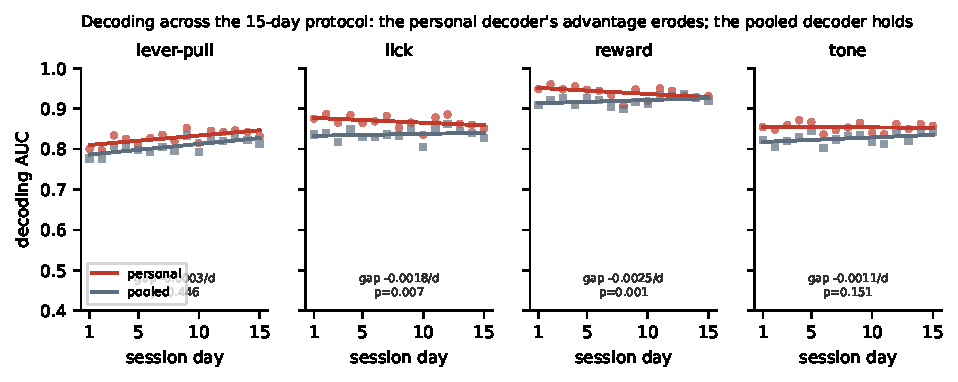
\includegraphics[width=0.98\linewidth]{figs/fig_decay.pdf}
\caption{Decoding accuracy across the 15-day protocol for the personal decoder (own early data) and
the pooled decoder (other mice's early data), with per-day points and linear fits. The personal
decoder starts ahead, and the pooled decoder gains more over days, so the gap between them narrows.
The narrowing is significant for lick and reward, the two events where the personal decoder also
loses accuracy over days, and is not significant for lever pull or tone. The per-event gap slope and
its $p$ (paired sign-flip over mice) are shown.}
\label{fig:decay}\end{figure}

\subsection{The robustness is not a data-volume artifact}
\label{sec:matched}
A pooled decoder contains $\sim$24$\times$ more training events than a personal decoder. Its
stability could therefore reflect data volume rather than pooling. We test this possibility with a
count-matched control (Fig.~\ref{fig:mech}, left). For each held-out mouse we set the training-set
size to the number of events in that mouse's early block, $n$, and compare three decoders: self,
trained on the mouse's own $n$ events; one, trained on $n$ events from one other mouse; and many,
trained on $n$ events drawn across the other 24 mice. All three are evaluated on the same
early-to-late change in the held-out mouse. The ordering is consistent across all four events;
averaged across targets, self ages by $+0.023$ $\auc$, one by $-0.006$, and many by $-0.012$. At the
same sample count, the self decoder therefore ages $+0.029$ more than a decoder trained on one other
mouse. Data volume cannot explain this gap. Instead, the mouse's early-week decoder appears to fit
idiosyncratic features that later drift, while a decoder trained on another mouse does not have
access to those features. Pooling across many mice yields a further $-0.006$ relative to one mouse
(many $<$ one for all four events), so cross-individual diversity provides a smaller, additional
benefit.

\subsection{Diversity: a secondary scaling with the number of training individuals}
\label{sec:scaling}
We next vary the number of training mice, $N \in \{1, 2, 4, 8, 16, 24\}$ (Fig.~\ref{fig:mech},
right). As $N$ increases, pooled aging becomes slightly more favorable for lick ($-0.001$ to
$-0.010$), reward ($-0.004$ to $-0.010$), and tone ($+0.003$ to $-0.010$). Lever-pull performance
saturates with a single training mouse and remains near $-0.025$. This scaling effect is modest,
approximately $0.01$ $\auc$ compared with the approximately $0.03$ self-versus-other gap. Most of the
resistance to drift is therefore present when training on only one other individual; additional
individuals provide a smaller refinement.

\begin{figure}[t]\centering
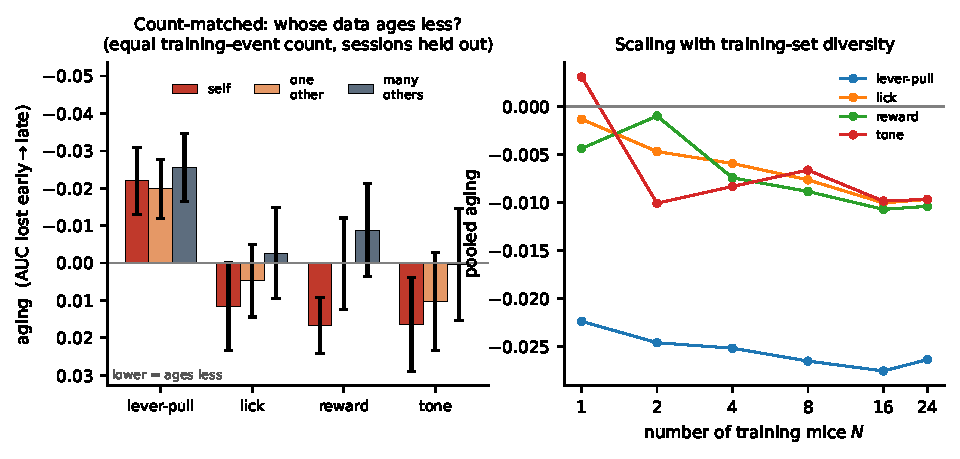
\includegraphics[width=0.98\linewidth]{figs/fig_mechanism.pdf}
\caption{\textbf{Left:} count-matched control. With equal numbers of training events, decoder aging
(AUC lost from early to late; lower values indicate greater robustness) is compared for the subject's
own data (self), one other mouse, and many other mice. The self decoder ages, whereas the
other-individual decoders do not. \textbf{Right:} pooled aging as a function of the number of
training mice $N$. Greater diversity provides a small additional gain, with immediate saturation for
lever pull.}
\label{fig:mech}\end{figure}

\subsection{The effect does not depend on the decoder}
\label{sec:nl}
Every aging number so far comes from a linear decoder. A higher-capacity decoder could overfit the
subject's early sessions more, which would enlarge the effect, or it could exploit fine temporal
structure that averages out the effect. We recompute the personal-minus-pooled aging asymmetry with
a 1-D CNN and a GRU over the full evoked window, on the same events and blocks (Table~\ref{tab:nl}).
The asymmetry stays positive and significant under every decoder and every event: the personal
decoder ages more than the pooled one under the linear model, the CNN, and the GRU alike. For lever
pull and tone the gap widens with the nonlinear decoders (CNN asymmetry $+0.088$ and $+0.061$),
consistent with a higher-capacity decoder fitting the subject's drift-prone features more closely;
for lick and reward it is comparable across decoders. The drift-resistance is therefore a property
of the code, not of the linear readout.

\begin{table}[t]\centering
\caption{Personal-minus-pooled aging asymmetry under three decoders, per event, $n = 25$ mice. A
positive value means the personal decoder ages more. Every cell is positive and significant; for
lever pull and tone the effect is larger with the nonlinear decoders. $p$: paired sign-flip
permutation. So that the three decoders differ only in capacity, all of them here use a single
80/20 split of the early block (the personal decoder trains on the 80\%), rather than the five-fold
estimate of Table~\ref{tab:asym}; this is why the linear column differs from Table~\ref{tab:asym} by
up to $0.002$ $\auc$.}
\label{tab:nl}
\setlength{\tabcolsep}{5pt}
\begin{tabular}{lccc}
\toprule
Event & Linear & 1-D CNN & GRU \\
\midrule
Lever-pull & $+0.016$ ($0.020$) & $+0.088$ ($<\!10^{-4}$) & $+0.057$ ($<\!10^{-4}$) \\
Lick       & $+0.033$ ($0.0003$) & $+0.028$ ($<\!10^{-4}$) & $+0.026$ ($<\!10^{-4}$) \\
Reward     & $+0.031$ ($0.0007$) & $+0.028$ ($0.0001$) & $+0.019$ ($0.002$) \\
Tone       & $+0.027$ ($0.009$) & $+0.061$ ($<\!10^{-4}$) & $+0.032$ ($0.002$) \\
\bottomrule
\end{tabular}
\end{table}

\section{Discussion}
A subject's own decoder overfits idiosyncratic features of its early sessions, some of which later
drift. A decoder that has never seen the subject must instead rely on components of the code that are
shared across individuals and more stable over time. The count-matched control supports this reading
directly: at equal data, other-individual data ages far less than the subject's own, and the effect
survives a nonlinear decoder that has more capacity to overfit. Population structure is therefore not
only a resource for cross-subject transfer, but also for temporal robustness. The initial accuracy
cost of cross-subject decoding is recovered over time as the pooled decoder remains stable. Unlike
within-subject recalibration, this approach does not require newly labelled data from the individual
at test time.

\textbf{Limitations.} We measure the effect at the mesoscale, using parcel-averaged activity. Whether
the same result holds for single-neuron codes, where representational drift is well characterized,
remains unknown. The analysis also covers four discrete task events, a two-week interval, and one
species; longer time periods, graded behaviors, other species, and other recording modalities should
be tested. Our conclusions depend on within-versus-pooled and early-versus-late comparisons rather
than on absolute $\auc$. Finally, although the count-matched control rules out training-set size and
is consistent with self-overfitting, it does not identify which components of drift are
individual-specific, and the additional effect of cross-individual diversity is small.

\subsubsection*{Reproducibility}
BraiDyn-BC is publicly available through DANDI:001425. We release the analysis code and a streaming
feature pipeline that reproduces all reported results from the parcellated traces without downloading
the raw imaging data. Section 3 and the released code specify all data splits, permutation seeds, and
hyperparameters.

{\small
\bibliographystyle{plainnat}
\begin{thebibliography}{99}
\bibitem[Degenhart et al.(2020)]{degenhart2020} A.~D.~Degenhart et al. Stabilization of a
brain--computer interface via the alignment of low-dimensional spaces of neural activity.
\emph{Nature Biomedical Engineering}, 4:672--685, 2020.
\bibitem[Driscoll et al.(2017)]{driscoll2017} L.~N.~Driscoll et al. Dynamic reorganization of
neuronal activity patterns in parietal cortex. \emph{Cell}, 170(5):986--999, 2017.
\bibitem[Farshchian et al.(2019)]{farshchian2019} A.~Farshchian et al. Adversarial domain
adaptation for stable brain--machine interfaces. \emph{ICLR}, 2019.
\bibitem[Jarosiewicz et al.(2015)]{jarosiewicz2015} B.~Jarosiewicz et al. Virtual typing by people
with tetraplegia using a self-calibrating intracortical brain--computer interface. \emph{Science
Translational Medicine}, 7(313):313ra179, 2015.
\bibitem[Kondo et al.(2025)]{kondo2025} A.~Kondo et al. BraiDyn-BC: a cortex-wide widefield calcium
imaging dataset during a cued lever-pull operant task. \emph{Scientific Data}, 12, 2025.
DANDI:001425.
\bibitem[MacDowell \& Buschman(2020)]{macdowell2020} C.~J.~MacDowell and T.~J.~Buschman.
Low-dimensional spatiotemporal dynamics underlie cortex-wide neural activity. \emph{Current
Biology}, 30(14):2665--2680, 2020.
\bibitem[MacDowell et al.(2024)]{macdowell2024} C.~J.~MacDowell et al. Shared cortex-wide
spatiotemporal motifs govern activity across individuals and behavioral states. \emph{Current
Biology}, 34, 2024.
\bibitem[Melbaum et al.(2022)]{melbaum2022} S.~Melbaum et al. Conserved structures of neural
activity in sensorimotor cortex of freely moving rats enable cross-subject decoding. \emph{Nature
Communications}, 13:7902, 2022.
\bibitem[Musall et al.(2019)]{musall2019} S.~Musall et al. Single-trial neural dynamics are
dominated by richly varied movements. \emph{Nature Neuroscience}, 22(10):1677--1686, 2019.
\bibitem[Peterson et al.(2021)]{peterson2021} S.~M.~Peterson, Z.~Steine-Hanson, N.~Davis,
R.~P.~N.~Rao, and B.~W.~Brunton. Generalized neural decoders for transfer learning across
participants and recording modalities. \emph{Journal of Neural Engineering}, 18:026014, 2021.
\bibitem[Karpowicz et al.(2025)]{karpowicz2025} B.~M.~Karpowicz, Y.~H.~Ali, L.~N.~Wimalasena,
et al. Stabilizing brain--computer interfaces through alignment of latent dynamics (NoMAD).
\emph{Nature Communications}, 16:4662, 2025.
\bibitem[Wilson et al.(2025)]{wilson2025} G.~H.~Wilson et al. Long-term unsupervised recalibration
of cursor-based intracortical brain--computer interfaces using a hidden Markov model. \emph{Nature
Biomedical Engineering}, 2025.
\bibitem[Rule et al.(2019)]{rule2019} M.~E.~Rule, T.~O'Leary, and C.~D.~Harvey. Causes and
consequences of representational drift. \emph{Current Opinion in Neurobiology}, 58:141--147, 2019.
\bibitem[Rule et al.(2020)]{rule2020} M.~E.~Rule et al. Stable task information from an unstable
neural population. \emph{eLife}, 9:e51121, 2020.
\bibitem[Schneider et al.(2023)]{schneider2023} S.~Schneider, J.~H.~Lee, and M.~W.~Mathis.
Learnable latent embeddings for joint behavioural and neural analysis (CEBRA). \emph{Nature},
617:360--368, 2023.
\bibitem[Schoonover et al.(2021)]{schoonover2021} C.~E.~Schoonover et al. Representational drift in
primary olfactory cortex. \emph{Nature}, 594:541--546, 2021.
\bibitem[Hosseini et al.(2026)]{wicat2026} M.~Hosseini, E.~Erturk, S.~Hashemi, and M.~M.~Shanechi.
Cross-subject modeling for widefield calcium imaging via atlas-aligned spatiotemporal tokenization.
In \emph{Proceedings of the 43rd International Conference on Machine Learning (ICML)}, 2026.
arXiv:2607.09754.
\end{thebibliography}
}

\end{document}
